\section{Component Diagram cho Task Assignment Module}
    \begin{figure}[h]
        \centering
        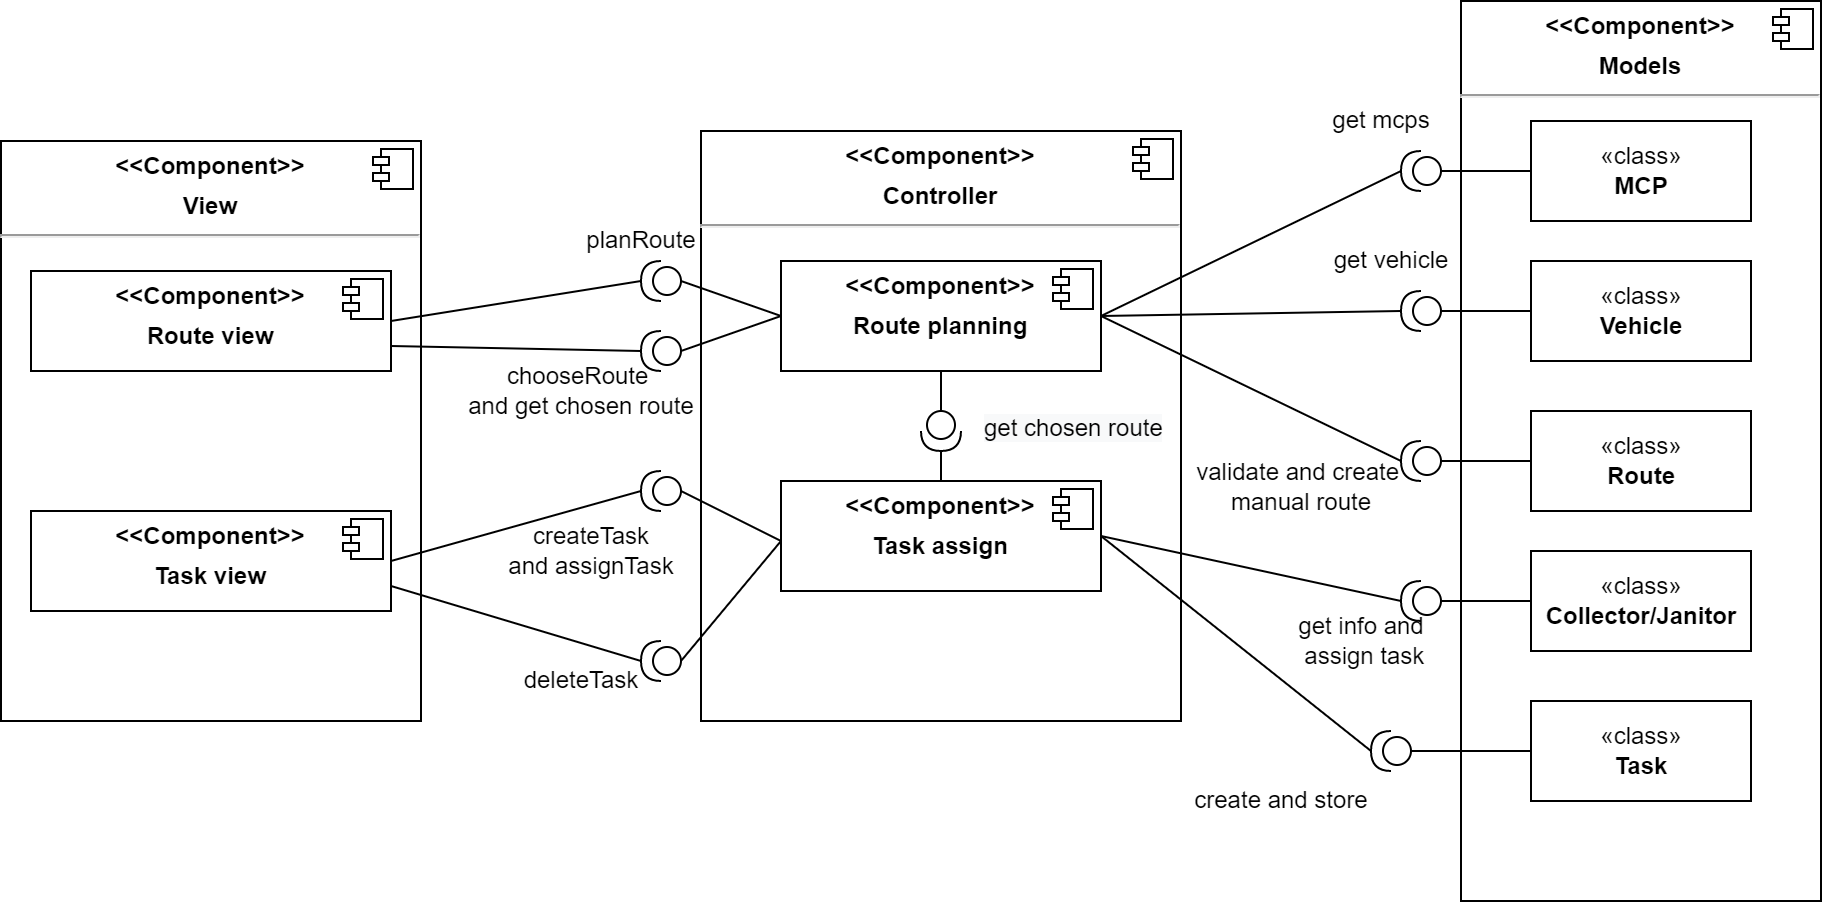
\includegraphics[width=1\linewidth]{imgs/component diagram/component Task Assignment.png}
        \caption{Component diagram cho task assignment module}
    \end{figure}
    Component diagram phía trên gồm ba component chính gồm View, Controller và Models:
    \begin{enumerate}
        \item Back officer-người thực hiện assgin task chỉ tương tác qua View component, trong đó:
        \begin{itemize}
            \item Route view dùng để thiết lập tuyến đường
            \item Task view sẽ dùng để tạo và gán task sau khi đã thiết lập tuyến đường xong
        \end{itemize}
        \item Lần lượt các tác vụ cho tuyến đường sẽ do Route planning controller thực hiện nhờ vào các class mang thông tin tính toán trong Models và tạo đối tượng Route để trả về cho view
        \item Tương tự như vậy cho Task assign controller, task assign controller cũng lấy thông tin tuyến đường đã lập và từ class Collector/Janitor để tạo các đối tượng Task và gán lại cho Collector/Janitor được chọn assign
    \end{enumerate}